\documentclass[twocolumn]{article}
\usepackage[utf8]{inputenc}
\usepackage[margin=1in]{geometry}  % 调整页面边距
\usepackage{titling}               % 控制标题位置
\usepackage{booktabs}              % 表格宏包
\usepackage{amssymb}
\usepackage{ctex}                  % 中文支持包
\usepackage{authblk}			   % 多作者
\usepackage{graphicx}
% \usepackage{xeCJK}
\setlength{\droptitle}{-3.0cm}     % 将标题上移3.0厘米

\title{Medical Image Classification using Support Vector Machine}
\author[1] {Your Name}
\author[1] {Teacher Author}
% \author[1,3]{Third Author}
\affil[1]{University of Fukui, 3-9-1 Bunkyo, Fukui, 910-0019, Japan}
% \affil[2]{Department of Electrical Engineering, University of Y}
% \affil[3]{Research Institute, Company Z}
\date{2024.11.30}

\begin{document}

\twocolumn[
	\maketitle

	\begin{center}
		\begin{abstract}
			This is Abstract chapter.
		\end{abstract}
	\end{center}
	\vspace{0.5cm}  % 调整摘要与正文之间的间距
]

\section{引言}
支持向量机(SVM)是一种强大的监督式学习算法,广泛应用于分类和回归任务中。该算法通过在特征空间中寻找最大间隔超平面来区分不同类别,有效地提高了模型的泛化能力。

\section{相关工作}
支持向量机早已被应用于文本分类任务中,如垃圾邮件检测和网页分类\cite{hearst_support_1998}。在人脸识别、手写识别\cite{bahlmann_online_2002}和医学图像分析\cite{gautam_investigation_2021}等领域,由于其高效的分类能力,SVM得到了广泛应用。支持向量机的发展与应用是机器学习领域中一个成功的案例,展示了理论研究如何被转化为实际应用的有效工具。

\section{方法}
本研究的目标是利用支持向量机(SVM)进行分类任务,找到一个能够最大化地分隔不同类别数据点的决策边界,即超平面。该超平面的表达式为:
\[
	f(x) = \mathbf{W}^\mathbb{T} x + b
\]
其中,\(f(x)\) 是模型的预测输出,表示样本 \(x_i\) 落在特定类别的置信度。\( \mathbf{W} \) 是超平面的法向量,\( b \) 是偏置项,\( x \) 是输入的特征向量。

SVM通过解决一个优化问题来确定最优的\( \mathbf{W} \)和\( b \),该问题旨在最大化两个类别之间的间隔。通常使用合页损失(Hinge Loss)来训练分类器,该损失函数鼓励找到具有最大边缘的决策边界,定义为:
\[
	L(y_i, f(x_i)) = \max(0, 1 - y_i f(x_i))
\]
其中,\( f(x_i) = \mathbf{W}^\mathbb{T} x_i + b \),\( y_i \) 是实际的类标签,取值为 \{-1, 1\}。
本研究构建了一个基本的支持向量机,利用合页损失对其进行优化,实现一个医学图像分类器。

\section{实验}
本研究利用SVM对医学图像进行分类,判断图像是PET还是CT。该数据集来源于国家癌症研究院的癌症成像计划(CIP),涵盖了355名受试者的肺部扫描图像,共251135张扫描图\cite{li_large-scale_2020}。这些图像主要收集自2009年至2011年间,每位受试者的数据包括性别、年龄、体重、吸烟史及癌症诊断分类。所有扫描数据以DICOM格式存储。本实验选取了38名被诊断为小细胞癌的受试者的数据,这部分数据包括PET扫描、多种CT扫描以及融合增强后的扫描图像,共12930张图像。通过精确筛选,获得了928张配对扫描图像用于本研究。

% 插入数据划分表格
\begin{table}[h]
	\centering
	\caption{实验数据划分}
	\label{tab:dataset_partition_1}
	\begin{tabular}{ccc}
		\toprule
		参数数量 & 测试数据集 & 训练数据集 \\
		\midrule
		肺部PET & 24 & 440 \\
		肺部CT & 24 & 440 \\
		总计 & 48 & 880 \\
		\bottomrule
	\end{tabular}
\end{table}

% 插入参数数量表格
\begin{table}[h]
	\centering
	\caption{不同输入图像尺寸下SVM决策函数需优化的参数数量}
	\label{tab:params_count}
	\begin{tabular}{cccc}
		\toprule
		参数数量 & 128×128 & 256×256 & 512×512 \\
		\midrule
		通道=1 & 16385 & 65537 & 262145 \\
		通道=2 & 32769 & 131073 & 524289 \\
		通道=3 & 49153 & 196609 & 786433 \\
		\bottomrule
	\end{tabular}
\end{table}

% 插入损失和准确率图表
\begin{figure}[h]
    \centering
    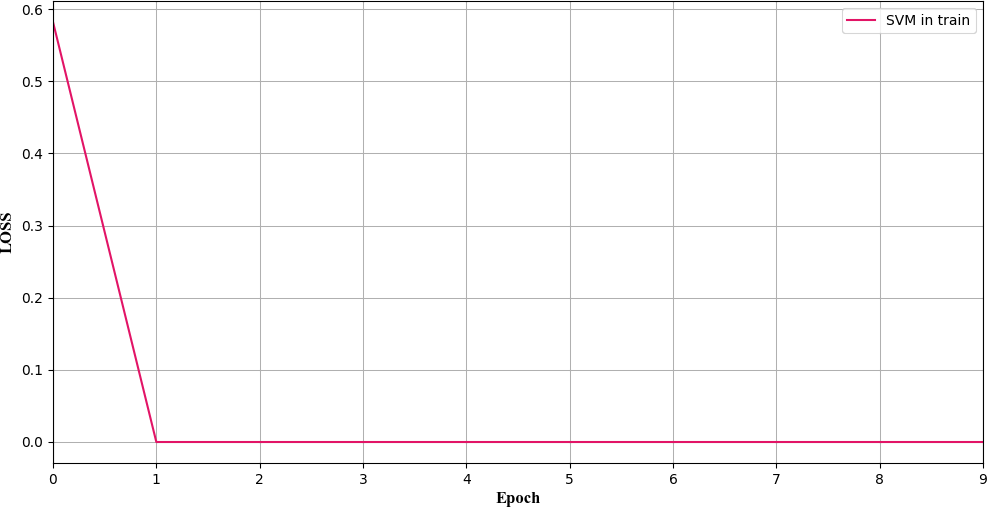
\includegraphics[width=1.0\linewidth]{exp_log/train440_valid024/LOSS_train}
    \caption{训练过程中各周期的损失变化图}
    \label{fig:loss_train}
\end{figure}

\begin{figure}[h]
    \centering
    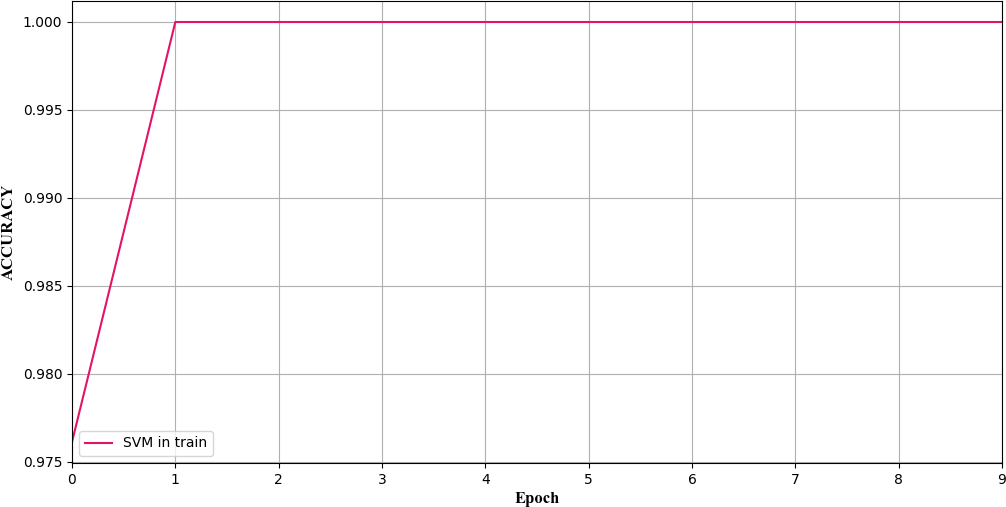
\includegraphics[width=1.0\linewidth]{exp_log/train440_valid024/ACCURACY_train}
    \caption{训练集上各周期的准确率变化图}
    \label{fig:acc_train}
\end{figure}

\begin{figure}[h]
    \centering
    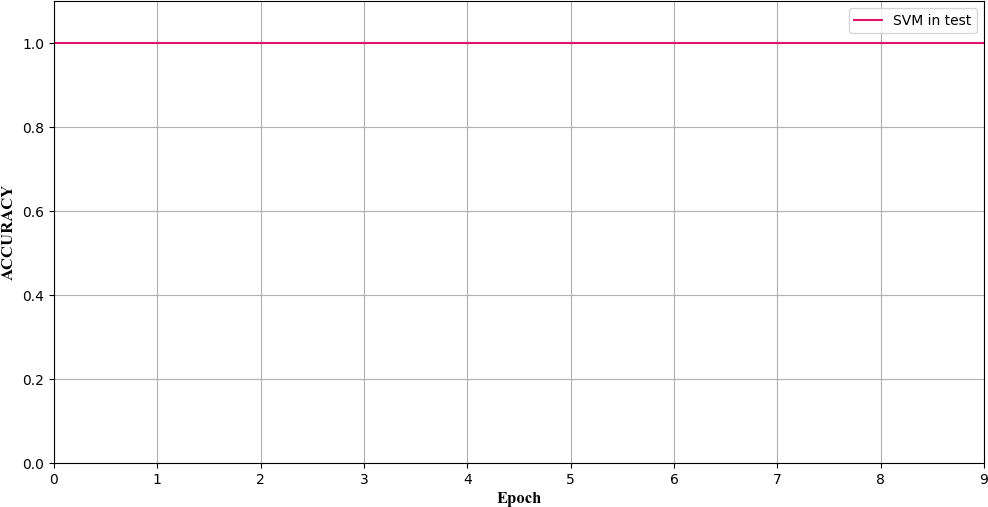
\includegraphics[width=1.0\linewidth]{exp_log/train440_valid024/ACCURACY_test}
    \caption{测试集上各周期的准确率变化图}
    \label{fig:acc_test}
\end{figure}

\section{结论}
本研究深入探讨了支持向量机的发展历史、技术原理及其在医学图像分类任务中的应用。实验结果显示,使用本研究中的数据集对SVM进行训练和测试,模型不仅能有效完成分类任务,而且显示出优异的分类性能。

\section*{致谢}
本文对国家癌症研究院癌症成像计划表示感谢,感谢其在互联网上公开并授权使用其高质量的医疗图像数据集,为本研究的顺利进行提供了重要资源。


\bibliographystyle{unsrt}
\bibliography{svm}

\end{document}
